\chapter{Appendix}\label{chapter:appendix}

\section{example of autopatch triple}\label{chapter:appendix_example_autopatch}

input vulnerable code
\begin{lightcpp}
    static void hsw_enable_crt(struct intel_atomic_state *state,
struct intel_encoder *encoder,
const struct intel_crtc_state *crtc_state,
const struct drm_connector_state *conn_state)
{
// Convert the atomic state to an intel_display structure
struct intel_display *display = to_intel_display(state);
// Convert the encoder's base device to a drm_i915_private structure
struct drm_i915_private *dev_priv = to_i915(encoder->base.dev);
// Convert the CRTC state to an intel_crtc structure
struct intel_crtc *crtc = to_intel_crtc(crtc_state->uapi.crtc);
// Retrieve the pipe associated with the CRTC
enum pipe pipe = crtc->pipe;
// Warn if the CRTC state does not have a PCH encoder
drm_WARN_ON(&dev_priv->drm, !crtc_state->has_pch_encoder);
// Enable the transcoder function for the encoder
intel_ddi_enable_transcoder_func(encoder, crtc_state);
// Enable the transcoder for the CRTC state
intel_enable_transcoder(crtc_state);
// Enable the PCH for the given state and CRTC
lpt_pch_enable(state, crtc);
// Enable vblank for the CRTC state
intel_crtc_vblank_on(crtc_state);
// Set the DPMS mode to ON for the encoder and CRTC state
intel_crt_set_dpms(encoder, crtc_state, DRM_MODE_DPMS_ON);
// Wait for the next vblank event on the CRTC
intel_crtc_wait_for_next_vblank(crtc);
// Wait for another vblank event on the CRTC
intel_crtc_wait_for_next_vblank(crtc);
// Enable CPU FIFO underrun reporting for the given pipe
intel_set_cpu_fifo_underrun_reporting(dev_priv, pipe, true);
// Enable PCH FIFO underrun reporting for PIPE_A
intel_set_cpu_fifo_underrun_reporting(dev_priv, PIPE_A, true);
}
\end{lightcpp}
ground truth

\begin{lightcpp}
struct intel_atomic_state;
struct intel_encoder {
    struct {
        void *dev;
    } base;
};
struct intel_crtc_state {
    struct {
        void *crtc;
    } uapi;
    int has_pch_encoder;
};
struct drm_connector_state;
struct intel_display;
struct drm_i915_private {
    void *drm;
};
struct intel_crtc {
    enum pipe {
        PIPE_A,
        PIPE_B,
        PIPE_C
    } pipe;
};

static struct intel_display* to_intel_display(struct intel_atomic_state *state) {
    return 0;
}

static struct drm_i915_private* to_i915(void *dev) {
    return 0;
}

static struct intel_crtc* to_intel_crtc(void *crtc) {
    return 0;
}

static void drm_WARN_ON(void *drm, int condition) {}

static void intel_ddi_enable_transcoder_func(struct intel_encoder *encoder, const struct intel_crtc_state *crtc_state) {}

static void intel_enable_transcoder(const struct intel_crtc_state *crtc_state) {}

static void lpt_pch_enable(struct intel_atomic_state *state, struct intel_crtc *crtc) {}

static void intel_crtc_vblank_on(const struct intel_crtc_state *crtc_state) {}

static void intel_crt_set_dpms(struct intel_encoder *encoder, const struct intel_crtc_state *crtc_state, int mode) {}

static void intel_crtc_wait_for_next_vblank(struct intel_crtc *crtc) {}

static void intel_set_cpu_fifo_underrun_reporting(struct drm_i915_private *dev_priv, enum pipe pipe, int enable) {}

static void hsw_enable_crt(struct intel_atomic_state *state,
                           struct intel_encoder *encoder,
                           const struct intel_crtc_state *crtc_state,
                           const struct drm_connector_state *conn_state)
{
    struct intel_display *display = to_intel_display(state);
    struct drm_i915_private *dev_priv = to_i915(encoder->base.dev);
    struct intel_crtc *crtc = to_intel_crtc(crtc_state->uapi.crtc);
    enum pipe pipe = crtc->pipe;

    drm_WARN_ON(&dev_priv->drm, !crtc_state->has_pch_encoder);
    intel_ddi_enable_transcoder_func(encoder, crtc_state);
    intel_enable_transcoder(crtc_state);
    lpt_pch_enable(state, crtc);
    intel_crtc_vblank_on(crtc_state);
    intel_crt_set_dpms(encoder, crtc_state, 1); // Assuming 1 as DRM_MODE_DPMS_ON
    intel_crtc_wait_for_next_vblank(crtc);
    intel_crtc_wait_for_next_vblank(crtc);
    intel_set_cpu_fifo_underrun_reporting(dev_priv, pipe, 1); // Assuming true as 1
    intel_set_cpu_fifo_underrun_reporting(dev_priv, PIPE_A, 1); // Assuming true as 1
\}
}
\end{lightcpp}
patch generated by the pipeline 
\begin{lightcpp}
    static void hsw_enable_crt(struct intel_atomic_state *state,
struct intel_encoder *encoder,
const struct intel_crtc_state *crtc_state,
const struct drm_connector_state *conn_state)
{
// Convert the atomic state to an intel_display structure
struct intel_display *display = to_intel_display(&state->base);
// Convert the encoder's base device to a drm_i915_private structure
struct drm_i915_private *dev_priv = to_i915(encoder->base.dev);
// Convert the CRTC state to an intel_crtc structure
struct intel_crtc *crtc = to_intel_crtc(crtc_state->uapi.crtc);
// Retrieve the pipe associated with the CRTC
enum pipe pipe = crtc->pipe;
// Warn if the CRTC state does not have a PCH encoder
drm_WARN_ON(&dev_priv->drm, !crtc_state->has_pch_encoder);
// Enable the transcoder function for the encoder
intel_ddi_enable_transcoder_func(encoder, crtc_state);
// Enable the transcoder for the CRTC state
intel_enable_transcoder(crtc_state);
// Enable the PCH for the given state and CRTC
lpt_pch_enable(state, crtc);
// Enable vblank for the CRTC state
intel_crtc_vblank_on(crtc_state);
// Set the DPMS mode to ON for the encoder and CRTC state
intel_crt_set_dpms(encoder, crtc_state, DRM_MODE_DPMS_ON);
// Wait for the next vblank event on the CRTC
intel_crtc_wait_for_next_vblank(crtc);
// Wait for another vblank event on the CRTC
intel_crtc_wait_for_next_vblank(crtc);
// Enable CPU FIFO underrun reporting for the given pipe
intel_set_cpu_fifo_underrun_reporting(dev_priv, pipe, true);
// Enable PCH FIFO underrun reporting for PIPE_A
intel_set_cpu_fifo_underrun_reporting(dev_priv, PIPE_A, true);
}
\end{lightcpp}
\begin{figure}
    \centering
    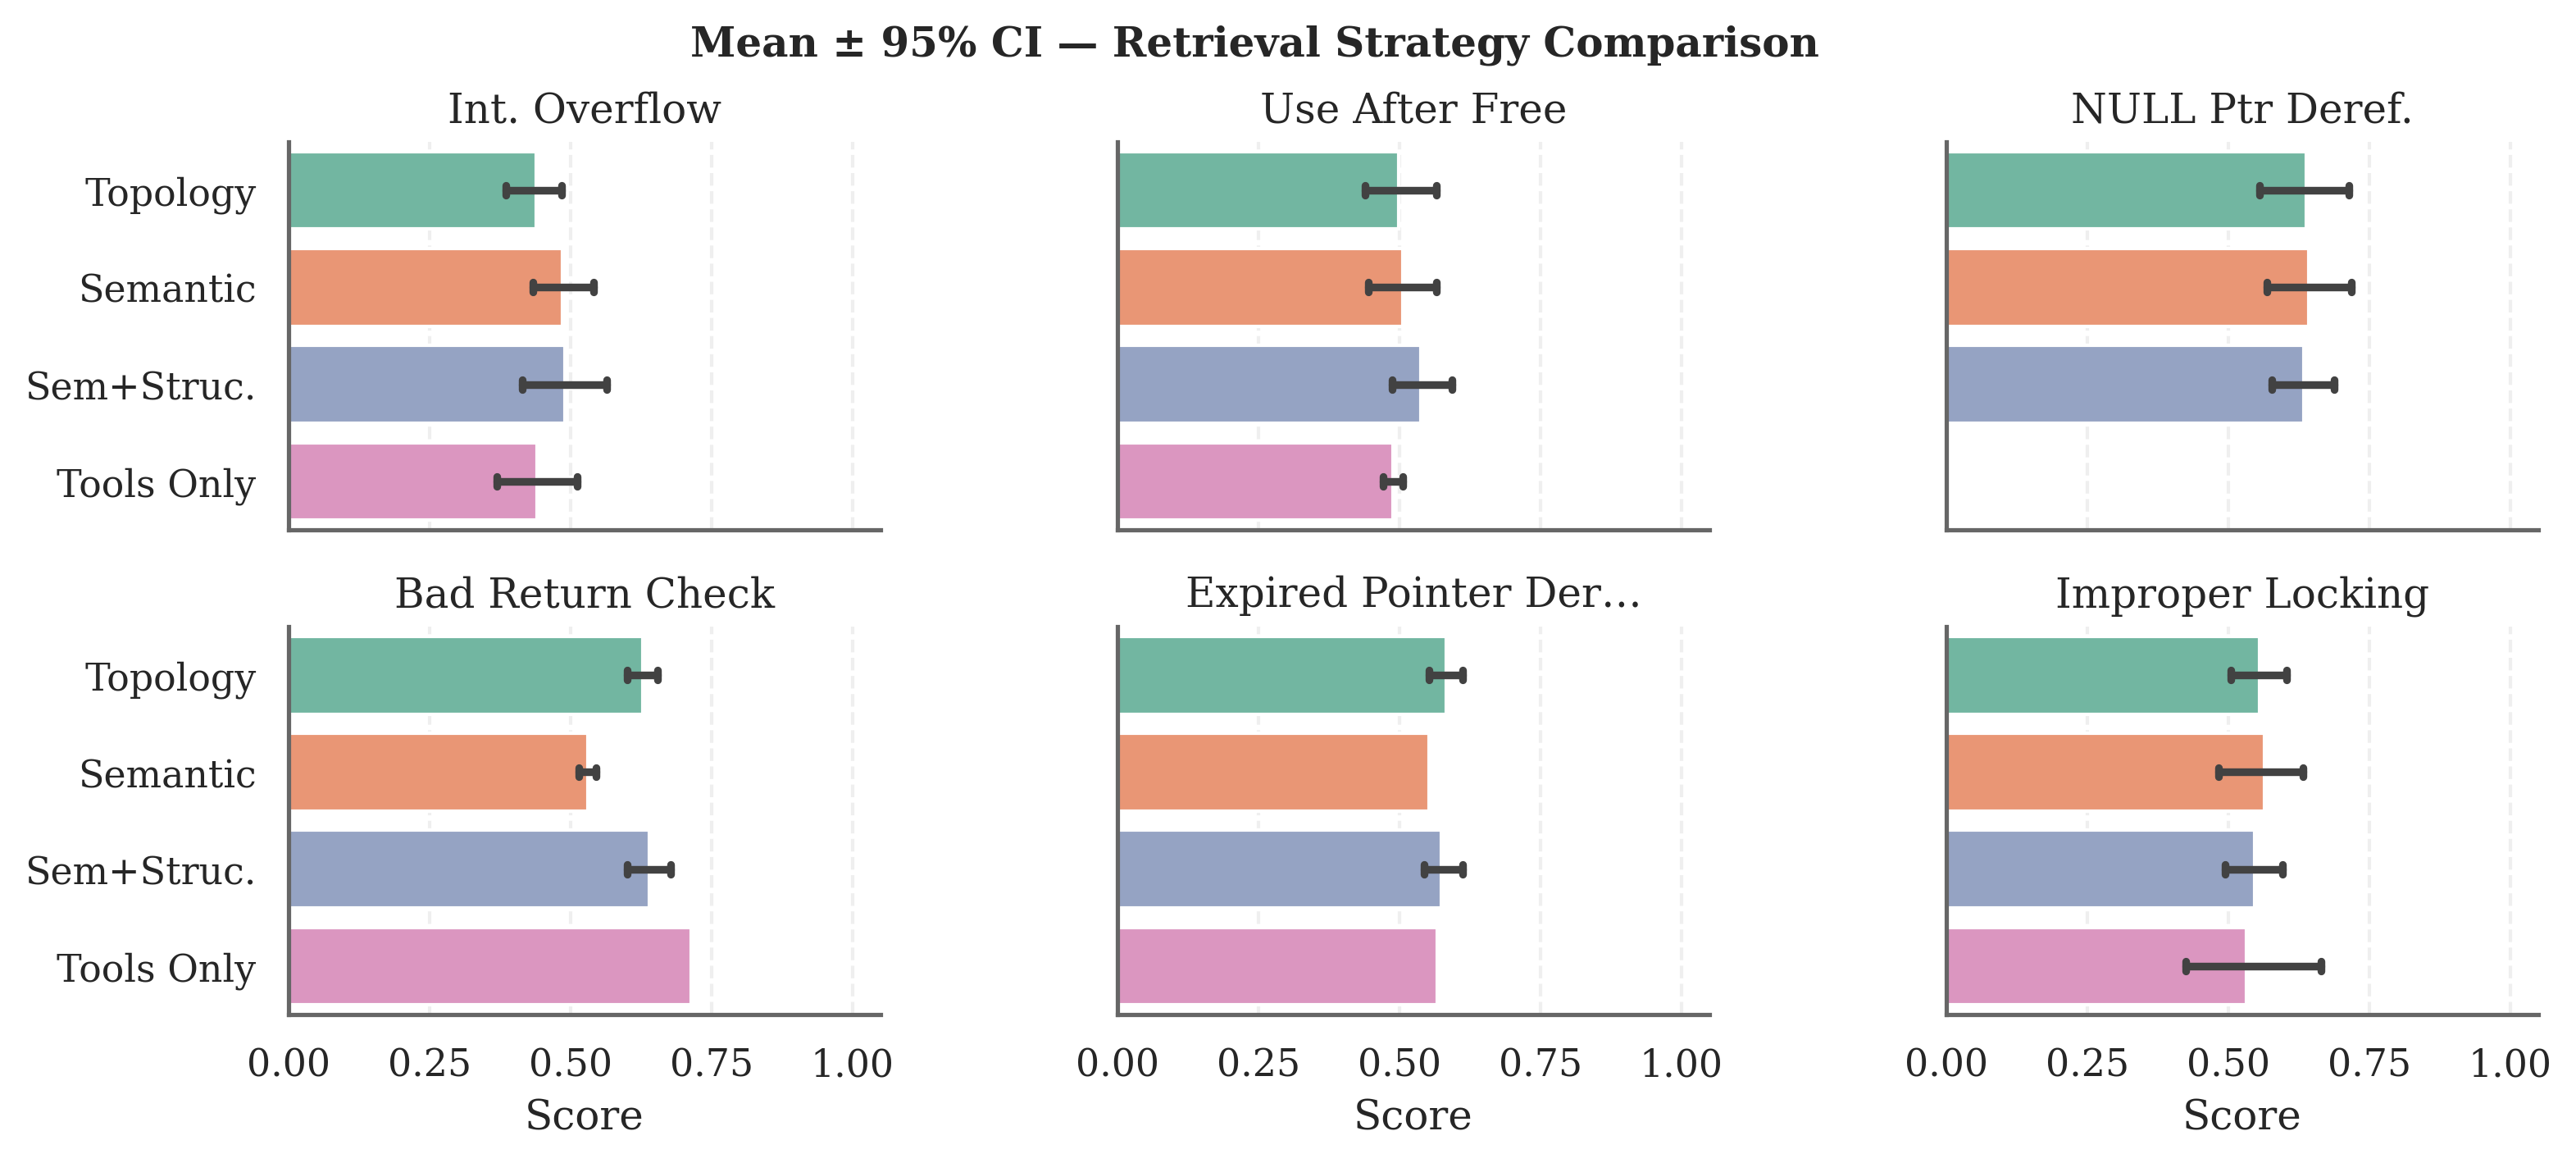
\includegraphics[width=1\linewidth]{img/patching/ci_gpt4_bertscore.png}
    \caption{BERTScore confidence intervals for GPT-4o patching on AutoPatch, grouped by CWE category.}
    \label{img:autopatch_gpt4o_bertscore}
\end{figure}
\begin{table}[H]
  \centering
  \caption{GPT-5.3-Codex: Overall pipeline performance on the autopatch dataset}
  \label{tab:autopatch_overall_pipeline_performance_gpt_codex}
  \begin{tabular}{lrrrrrr}
    \toprule
    Source & N & \makecell{Completion \\ \%} & BLEU-4 & BERTScore F1 & ROUGE-L F1 & \makecell{LLM\\ Judge\\ Valid} \\
    \midrule
    CodeBERT Pattern & 75 & 88.0 & 0.828 $\pm$ 0.000 & 0.525 $\pm$ 0.127 & 0.900 $\pm$ 0.106 & 70.3 \\
    CodeBERT Seq & 75 & 96.0 & 0.827 $\pm$ 0.000 & 0.527 $\pm$ 0.124 & 0.900 $\pm$ 0.100 & 82.7 \\
    Combined & 75 & 100.0 & 0.829 $\pm$ 0.000 & 0.521 $\pm$ 0.126 & 0.898 $\pm$ 0.100 & 85.3 \\
    \bottomrule
  \end{tabular}
\end{table}

\begin{table}[H]
  \centering
  \caption{GPT-5.3-Codex: Pipeline performance by CWE category on the autopatch dataset}
  \label{tab:autopatch_pipeline_by_cwe_category_gpt_codex}
  \begin{tabular}{llrrrr}
    \toprule
    Source & Category & N & BLEU-4 & BERTScore F1 & ROUGE-L F1 \\
    \midrule
    \multirow{4}{*}{CodeBERT Pattern} & Memory Safety & 22 & 0.842 & 0.539 & 0.917 \\\\
    & Concurrency & 28 & 0.799 & 0.518 & 0.867 \\
    & Numeric/Type & 10 & 0.865 & 0.314 & 0.911 \\
    & Resource Mgmt & 8 & 0.711 & 0.487 & 0.812 \\
    \midrule
    \multirow{4}{*}{CodeBERT Seq} & Memory Safety & 25 & 0.828 & 0.539 & 0.906 \\\\
    & Concurrency & 30 & 0.792 & 0.515 & 0.862 \\
    & Numeric/Type & 10 & 0.868 & 0.317 & 0.918 \\
    & Resource Mgmt & 7 & 0.743 & 0.515 & 0.831 \\
    \midrule
    \multirow{4}{*}{Combined} & Memory Safety & 26 & 0.830 & 0.537 & 0.902 \\\\
    & Concurrency & 31 & 0.804 & 0.514 & 0.873 \\
    & Numeric/Type & 11 & 0.889 & 0.315 & 0.931 \\
    & Resource Mgmt & 7 & 0.743 & 0.515 & 0.831 \\
    \midrule
    \bottomrule
  \end{tabular}
\end{table}
